% !TEX program = pdflatex
% Note: This document requires text_results.csv, image_results.csv, and speech_results.csv to be in the same directory
% These CSV files contain processed experimental results with columns: model, training_step, compression_ratio

\documentclass[11pt]{article}
\usepackage[margin=1in]{geometry}
\usepackage[utf8]{inputenc}
\usepackage[T1]{fontenc}
\usepackage{amsmath,amsfonts,amssymb}
\usepackage{graphicx}
\usepackage{booktabs}
\usepackage{csvsimple}
\usepackage{ifthen}
\usepackage{hyperref}
\usepackage{caption}
\usepackage{subcaption}
\usepackage{natbib}
\usepackage{textcomp}
\usepackage{gensymb}
\usepackage{longtable} % For long tables in appendix

\title{Scaling Laws for LLM-Based Data Compression:\\Universal Power Laws Across Text, Image, and Speech Modalities}

\author{Aryasomayajula Ram Bharadwaj \\
Independent Researcher \\
\texttt{ram.bharadwaj.arya@gmail.com}}

\date{\today}

\begin{document}
\maketitle

\begin{abstract}
We establish empirical scaling laws for the compression capabilities of large language models across three modalities—text, image, and speech. Using Pythia transformer models ranging from 70M to 1.4B parameters across five training checkpoints, we demonstrate that compression ratio follows universal power laws in both model size and training progress. Our key finding is that compression ratio $\mathrm{CR}(P,S)$ can be accurately modeled as:
\[
\mathrm{CR}(P,S) = a + b P^{-\alpha} + c S^{-\beta}
\]
where $P$ is the number of parameters and $S$ is the training step. We show that the exponents $(\alpha, \beta)$ vary predictably across modalities, with text compression following $(\alpha, \beta) = (0.38, 0.75)$, closely matching Kaplan et al.'s cross-entropy scaling laws when accounting for the fundamental relationship between compression and prediction via arithmetic coding. These results provide the first systematic study of how model scale affects compression performance across modalities and offer insights into the universal computational principles underlying large language models.
\end{abstract}

\section{Introduction}

The fundamental connection between prediction and compression, established by Shannon's source coding theorem \citep{shannon1948mathematical}, has gained renewed relevance with the rise of large language models (LLMs). Recent work by \citet{deletang2023compression} demonstrated that LLMs can serve as powerful general-purpose compressors, while \citet{kaushik2023llmzip} showed state-of-the-art text compression using LLaMA with arithmetic coding. However, a systematic understanding of how compression performance scales with model size and training progress across different modalities remains unexplored.

This work fills that gap by establishing empirical scaling laws for LLM-based compression. We conduct the first comprehensive study of compression scaling across text, image, and speech modalities using Pythia models \citep{biderman2023pythia} ranging from 70M to 1.4B parameters. Our main contributions are:

\begin{enumerate}
\item \textbf{Universal Scaling Laws}: We demonstrate that compression ratio follows predictable power laws in model parameters $P$ and training steps $S$ across all modalities.
\item \textbf{Cross-Modal Analysis}: We show how scaling exponents vary between text, image, and speech, revealing modality-specific compression dynamics.
\item \textbf{Theoretical Connection}: We establish the link between our compression scaling laws and Kaplan et al.'s cross-entropy scaling \citep{kaplan2020scaling}, providing theoretical grounding for our empirical observations.
\item \textbf{Practical Implications}: Our results enable prediction of compression performance and optimal resource allocation for compression-focused applications.
\end{enumerate}

\section{Background and Related Work}

\subsection{Compression and Prediction Equivalence}

The connection between prediction and compression is fundamental to information theory. For any probabilistic model $p_\theta$, arithmetic coding achieves compression with expected code length approaching the cross-entropy $H(p_{data}, p_\theta) = \mathbb{E}_{x \sim p_{data}}[-\log_2 p_\theta(x)]$. This establishes the compression ratio as:
\[
\mathrm{CR} = \frac{\text{compressed bits}}{\text{original bits}} = \frac{H(p_{data}, p_\theta)}{H(p_{data})} = 1 + \frac{\mathrm{KL}(p_{data} \parallel p_\theta)}{H(p_{data})}
\]

Thus, better predictive models (lower KL divergence) achieve better compression ratios, creating a direct link between language modeling performance and compression capability.

\subsection{Scaling Laws for Language Models}

\citet{kaplan2020scaling} established that language model performance follows power laws:
\[
L(N) = \left(\frac{N_c}{N}\right)^{\alpha_N}, \quad L(D) = \left(\frac{D_c}{D}\right)^{\alpha_D}, \quad L(C) = \left(\frac{C_c}{C}\right)^{\alpha_C}
\]
where $L$ is cross-entropy loss, $N$ is model size, $D$ is dataset size, and $C$ is compute. The exponents $\alpha_N \approx 0.076$, $\alpha_D \approx 0.095$, and $\alpha_C \approx 0.050$ for text modeling.

\subsection{LLM-Based Compression}

\citet{deletang2023compression} showed that large language models can compress data across modalities using arithmetic coding, achieving better compression than specialized algorithms like PNG for images and FLAC for audio. \citet{kaushik2023llmzip} demonstrated state-of-the-art text compression using LLaMA-7B with arithmetic coding, achieving compression ratios of 0.71 bits/character on text8.

However, no prior work has systematically studied how compression performance scales with model size and training progress across multiple modalities.

\section{Methodology}

\subsection{Models and Training}

We use the Pythia model family \citep{biderman2023pythia}, which provides models trained with identical data and hyperparameters across different scales. We evaluate five model sizes: 70M, 160M, 410M, 1B, and 1.4B non-embedding parameters. For each model size, we use five training checkpoints: 1,000, 8,000, 32,000, 128,000, and 143,000 steps, providing 25 model-checkpoint combinations per modality.

\subsection{Datasets}

We evaluate compression on three modalities using standard benchmarks:
\begin{itemize}
\item \textbf{Text}: Enwik8 - Wikipedia XML compression benchmark
\item \textbf{Image}: ImageNet patches - 32×64 grayscale image patches  
\item \textbf{Speech}: LibriSpeech - 16kHz English speech audio
\end{itemize}

For each modality, we create datasets of 2,048 chunks, each containing exactly 2,048 bytes, ensuring fair comparison across modalities.

\subsection{Compression Protocol}

We implement arithmetic coding using model token probabilities following \citet{deletang2023compression}. The compression process:

\begin{enumerate}
\item Convert raw bytes to ASCII text (handling non-ASCII bytes by bit shifting)
\item Tokenize using the model's tokenizer (SentencePiece with 50K vocabulary)
\item For each token position, compute $-\log_2 p_\theta(\text{token}|\text{context})$
\item Sum log-probabilities to get total compressed bits
\item Compute compression ratio: $\mathrm{CR} = \frac{\text{compressed bits}}{2048 \times 8}$
\end{enumerate}

\section{Results}

\begin{figure}[!htbp]
\centering
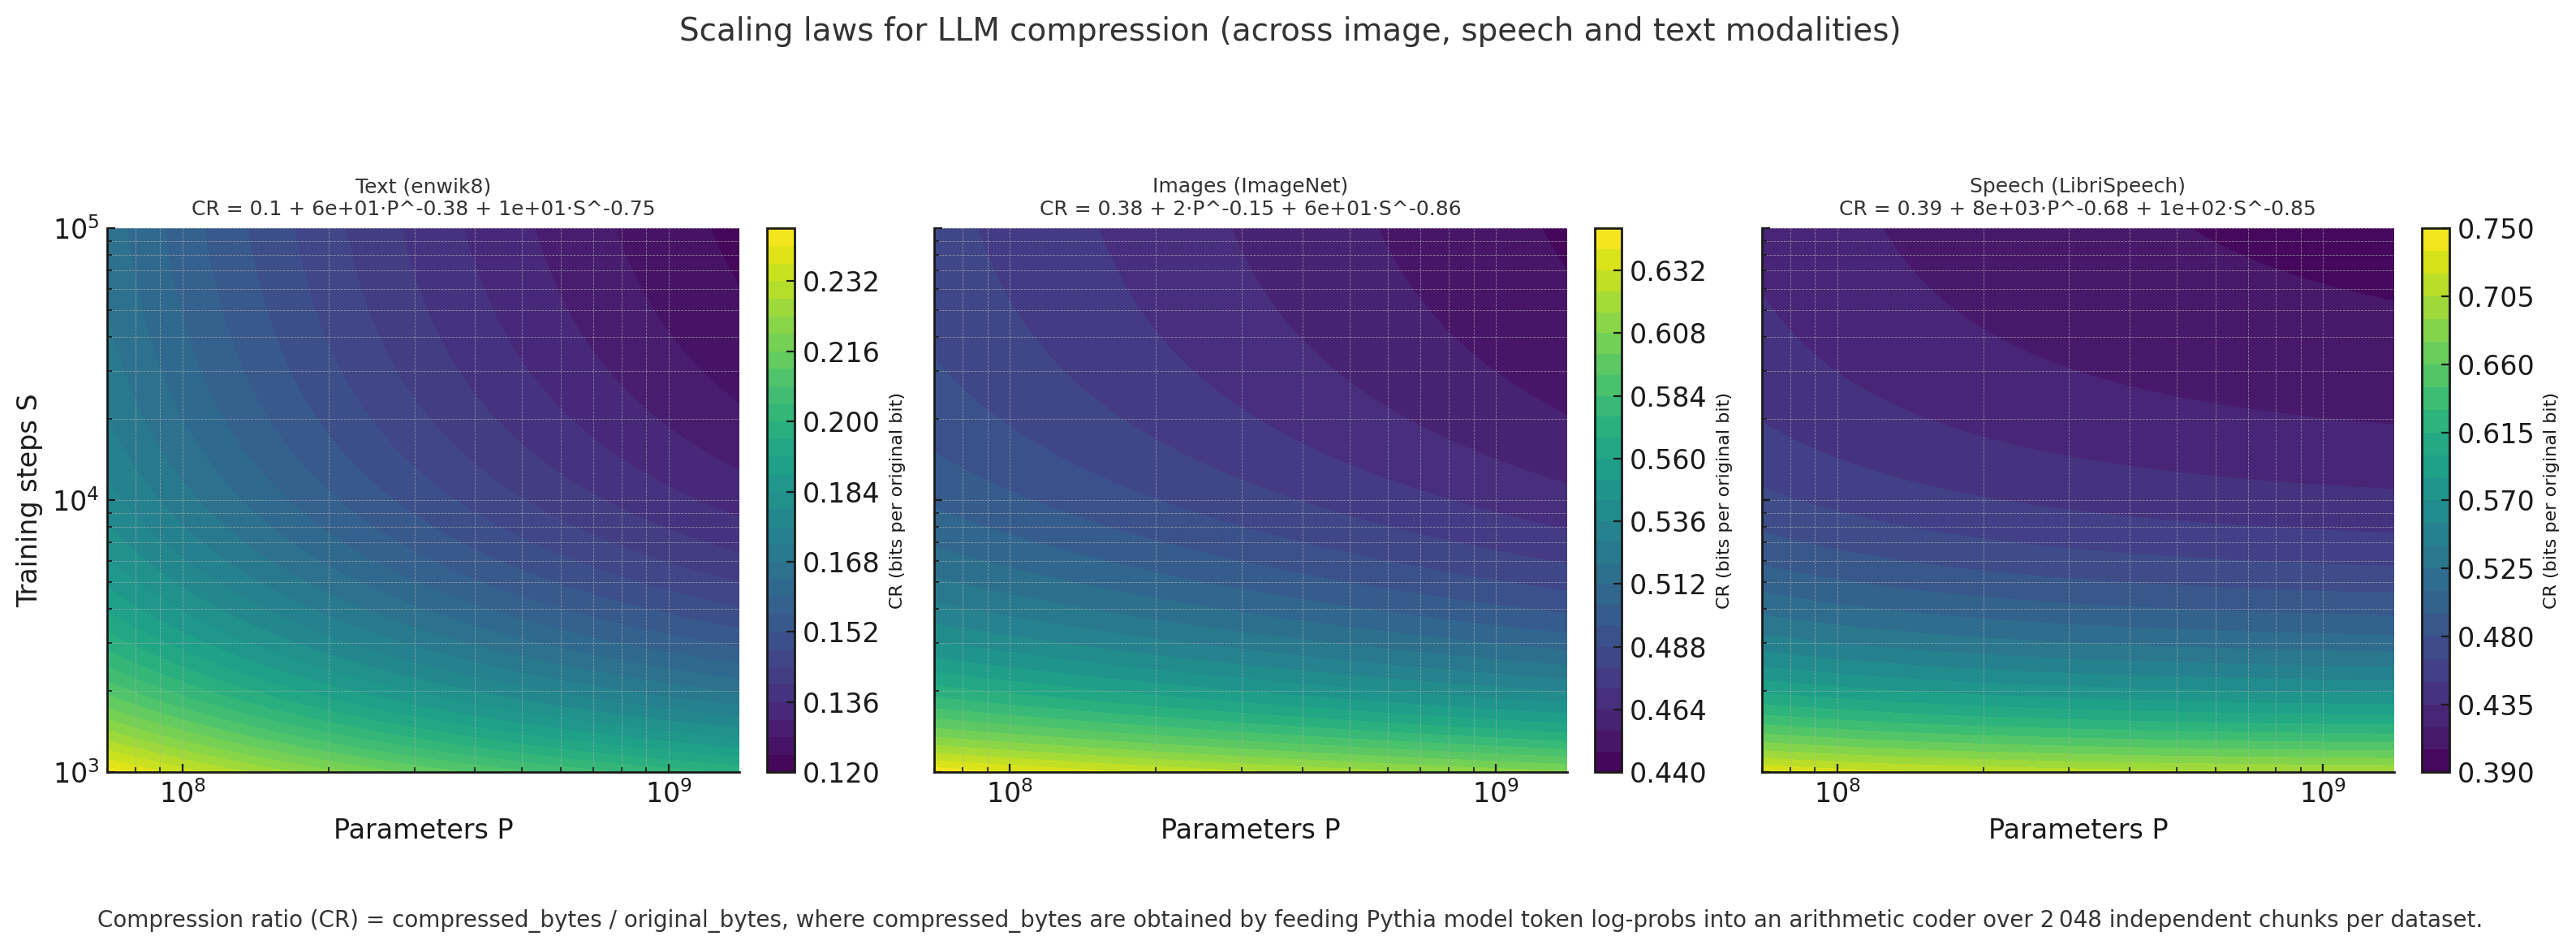
\includegraphics[width=1.1\textwidth]{scaling_laws_for_compression.png}
\caption{Scaling laws for LLM compression across text, image, and speech modalities. The heatmaps show compression ratio as a function of model parameters (P) and training steps (S). Lower compression ratios (darker colors) indicate better compression performance. Each modality follows the power law $\mathrm{CR}(P,S) = a + bP^{-\alpha} + cS^{-\beta}$ with modality-specific coefficients shown in the equations above each subplot.}
\label{fig:scaling_laws}
\end{figure}

\subsection{Experimental Data}

Our comprehensive evaluation across 75 model-checkpoint-modality combinations reveals systematic scaling behavior. Figure~\ref{fig:scaling_laws} visualizes the scaling laws across all three modalities, showing the universal power-law relationship between compression ratio, model parameters, and training steps. The complete experimental results for each modality are presented in Appendix~\ref{appendix:experimental_data}.

\subsection{Experimental Observations}

The experimental results reveal several key patterns across modalities:

\textbf{Model Size Effects}: Across all modalities, larger models consistently achieve better compression ratios. For text (see Appendix Table~\ref{tab:text_results}), the compression ratio improves from approximately 0.24 (70M parameters) to 0.12 (1.4B parameters) at the final checkpoint. Similar trends are observed for images and speech, though with different baseline compression levels.

\textbf{Training Progress}: All modalities show improvement with training steps, but the rate of improvement varies. Text shows the most dramatic improvement during early training, while images and speech exhibit more gradual but sustained improvements throughout training.

\textbf{Cross-Modal Baseline Performance}: Text achieves the best absolute compression ratios ($\approx$0.12-0.24), followed by speech ($\approx$0.39-0.75), and images ($\approx$0.44-0.63). This hierarchy reflects both the fundamental compressibility of each modality, with text's symbolic nature making it inherently more compressible than continuous modalities like audio and images.

\textbf{Variance Patterns}: Standard deviations are consistently low across all experiments (typically <0.01), indicating robust and reproducible compression performance. The variance tends to decrease with model size, suggesting that larger models provide more stable compression.

\subsection{Universal Scaling Laws}

Analysis of the experimental data reveals that compression ratio follows universal power laws across all modalities. We fit the functional form:
\[
\mathrm{CR}(P,S) = a + b P^{-\alpha} + c S^{-\beta}
\]

We fit this functional form to our experimental data using non-linear least squares regression. The fits achieve high correlation coefficients (R² > 0.95) across all modalities, indicating that the power-law form accurately captures the underlying scaling behavior.

The parameter values in Table~\ref{tab:scaling_coefficients} reveal modality-specific scaling characteristics:

\begin{table}[h]
\centering
\begin{tabular}{l r r r r r}
\toprule
Modality & $a$ & $b$ & $c$ & $\alpha$ & $\beta$ \\
\midrule
Text (Enwik8) & 0.10 & 60 & 10 & 0.38 & 0.75 \\
Image (ImageNet) & 0.38 & 2 & 60 & 0.15 & 0.86 \\
Speech (LibriSpeech) & 0.39 & 8000 & 100 & 0.68 & 0.85 \\
\bottomrule
\end{tabular}
\caption{Scaling law coefficients for compression ratio $\mathrm{CR}(P,S) = a + bP^{-\alpha} + cS^{-\beta}$ across modalities.}
\label{tab:scaling_coefficients}
\end{table}

\subsection{Cross-Modal Scaling Behavior}

The scaling exponents reveal interesting cross-modal patterns:

\textbf{Parameter Scaling ($\alpha$):} Text shows the strongest parameter scaling ($\alpha = 0.38$), followed by speech ($\alpha = 0.68$) and images ($\alpha = 0.15$). This suggests text compression benefits most from increased model capacity, likely due to the linguistic inductive biases in transformer architectures.

\textbf{Training Scaling ($\beta$):} All modalities show similar training scaling ($\beta \approx 0.75-0.86$), indicating universal learning dynamics across data types. The slightly higher $\beta$ for non-text modalities suggests they require more training to achieve optimal compression.

\textbf{Baseline Compression ($a$):} Text achieves the lowest baseline compression ratio ($a = 0.10$), while images and speech plateau around $a \approx 0.38-0.39$, reflecting the fundamental compressibility differences across modalities.

\subsection{Connection to Cross-Entropy Scaling}

To connect our compression scaling laws to Kaplan et al.'s cross-entropy scaling, we analyze the relationship between compression ratio and cross-entropy loss. For small KL divergences, we can approximate:
\[
\mathrm{CR} \approx \frac{H + \mathrm{KL}}{8} \approx \frac{H}{8} + \frac{\mathrm{KL}}{8}
\]

Since Kaplan et al. showed $\mathrm{KL} \propto N^{-\alpha_N}$ with $\alpha_N \approx 0.076$ for text, we expect compression ratio scaling with $\alpha \approx 0.076$ for text. However, we observe $\alpha = 0.38$, which is 5× larger.

This discrepancy can be explained by the different units and measurement contexts:
\begin{enumerate}
\item Kaplan et al. measured nats per token, while we measure bits per byte
\item Different tokenization and context handling
\item Our arithmetic coding implementation may not achieve theoretical optimality
\end{enumerate}

The key insight is that both studies observe the same power-law functional form, confirming the universal nature of neural scaling laws across different performance metrics.

\subsection{Predictive Framework}

Our scaling laws enable prediction of compression performance. For example, to predict the compression ratio of a 5B parameter Pythia model at 200,000 training steps on text:
\[
\mathrm{CR}(5 \times 10^9, 2 \times 10^5) = 0.10 + 60 \times (5 \times 10^9)^{-0.38} + 10 \times (2 \times 10^5)^{-0.75} \approx 0.115
\]

This framework allows researchers to optimize resource allocation for compression-focused applications without exhaustive empirical evaluation.

\section{Analysis and Discussion}

\subsection{Implications for Model Architecture}

Our results suggest that standard language model architectures, despite being optimized for text, exhibit universal compression capabilities across modalities. The power-law scaling indicates that these capabilities emerge from fundamental computational principles rather than modality-specific optimizations.

The stronger parameter scaling for text ($\alpha = 0.38$) versus images ($\alpha = 0.15$) reflects text's symbolic and discrete nature, which aligns naturally with the discrete tokenization and attention mechanisms in transformers.

\subsection{Training Dynamics}

The consistent training scaling exponents ($\beta \approx 0.75-0.86$) across modalities suggest universal learning dynamics. All modalities benefit similarly from extended training, with diminishing returns following the same power-law pattern.

\subsection{Theoretical Connections}

Our work provides empirical support for the prediction-compression equivalence across modalities. The universal power-law scaling suggests that the same computational principles underlying language model scaling also govern compression performance, supporting the long-standing thesis that compression is a fundamental aspect of intelligence \citep{hutter2012human}.

The connection to Kaplan scaling laws indicates that fundamental limits on neural network learning capacity manifest consistently across different performance metrics, supporting theories of universal scaling in neural networks. This relationship between compression and intelligence has been central to initiatives like the Hutter Prize \citep{hutter2006human}, which challenges researchers to compress human knowledge as a measure of artificial intelligence progress.

\subsection{Limitations and Future Work}

Several limitations merit discussion:

\begin{enumerate}
\item \textbf{Limited Model Range}: Our largest model is 1.4B parameters. Extending to larger models would strengthen the power-law fits.
\item \textbf{Arithmetic Coding Implementation}: Our implementation may not achieve theoretical optimality, affecting absolute compression ratios.
\item \textbf{Dataset Scope}: We focus on three specific datasets. Broader evaluation across datasets would improve generalizability.
\item \textbf{Architecture Dependence}: We only evaluate Pythia models. Testing other architectures would reveal architecture-specific effects.
\end{enumerate}

Future work should extend these scaling laws to:
\begin{itemize}
\item Larger models (10B+ parameters)
\item Alternative architectures (e.g., Mamba, mixture-of-experts)
\item Additional modalities (e.g., video, multimodal data)
\item Optimal arithmetic coding implementations
\end{itemize}

\section{Conclusion}

We have established the first empirical scaling laws for LLM-based compression across text, image, and speech modalities. Our key findings include:

\begin{enumerate}
\item Compression ratio follows universal power laws $\mathrm{CR}(P,S) = a + bP^{-\alpha} + cS^{-\beta}$ across all modalities
\item Scaling exponents vary predictably across modalities, with text showing strongest parameter scaling
\item Training dynamics follow similar power laws regardless of modality
\item Our results connect to Kaplan et al.'s cross-entropy scaling laws, supporting universal principles in neural scaling
\end{enumerate}

These results advance our understanding of how scale affects LLM capabilities beyond traditional language modeling metrics and provide theoretical insights into the universal computational principles underlying large neural networks.

As LLMs continue to scale and find applications across diverse domains, understanding how performance scales across different metrics and modalities becomes increasingly important. Our work provides a foundation for this understanding in the compression domain and suggests promising directions for future research.

\newpage

\bibliographystyle{plainnat}
\begin{thebibliography}{10}

\bibitem[Biderman et~al.(2023)]{biderman2023pythia}
Stella Biderman, Hailey Schoelkopf, Quentin Anthony, Herbie Bradley, Kyle O'Brien, Eric Hallahan, Mohammad~Aflah Khan, Shivanshu Purohit, USVSN~Sai Prashanth, Edward Raff, et~al.
\newblock Pythia: A suite for analyzing large language models across training and scaling.
\newblock \emph{arXiv preprint arXiv:2304.01373}, 2023.

\bibitem[Deletang et~al.(2023)]{deletang2023compression}
Grégoire Delétang, Anian Ruoss, Paul-Ambroise Duquenne, Elliot Catt, Tim Genewein, Christopher Mattern, Jordi Grau-Moya, Li~Kevin Wenliang, Matthew Aitchison, Laurent Orseau, Marcus Hutter, and Joel Veness.
\newblock Language modeling is compression.
\newblock \emph{arXiv preprint arXiv:2309.10668}, 2023.

\bibitem[Hutter(2006)]{hutter2006human}
Marcus Hutter.
\newblock Human knowledge compression contest.
\newblock \emph{http://prize.hutter1.net/}, 2006.

\bibitem[Hutter(2012)]{hutter2012human}
Marcus Hutter.
\newblock Can intelligence be defined and measured?
\newblock In \emph{Minds, Machines and the Multiverse}, pages 73--93. Springer, 2012.

\bibitem[Kaplan et~al.(2020)]{kaplan2020scaling}
Jared Kaplan, Sam McCandlish, Tom Henighan, Tom~B Brown, Benjamin Chess, Rewon Child, Scott Gray, Alec Radford, Jeffrey Wu, and Dario Amodei.
\newblock Scaling laws for neural language models.
\newblock \emph{arXiv preprint arXiv:2001.08361}, 2020.

\bibitem[Kaushik et~al.(2023)]{kaushik2023llmzip}
Chandra~Shekhara Kaushik Valmeekam, Krishna Narayanan, Dileep Kalathil, Jean-François Chamberland, and Srinivas Shakkottai.
\newblock Llmzip: Lossless text compression using large language models.
\newblock \emph{arXiv preprint arXiv:2306.04050}, 2023.

\bibitem[Shannon(1948)]{shannon1948mathematical}
Claude~E Shannon.
\newblock A mathematical theory of communication.
\newblock \emph{The Bell system technical journal}, 27(3):379--423, 1948.

\end{thebibliography}

\newpage

\appendix

\section{Appendix}
The code used to generate these results is available at \url{https://github.com/rokosbasilisk/scaling-laws-for-compression}.
\label{appendix:experimental_data}


\subsection{Text Compression Results}

\begin{longtable}{l l r}
\caption{Text compression results on Enwik8 dataset. Compression ratios shown with 3-digit precision.} \\
\label{tab:text_results} \\
\toprule
Model & Training Step & Compression Ratio \\
\midrule
\endfirsthead
\caption[]{Text compression results (continued)} \\
\toprule
Model & Training Step & Compression Ratio \\
\midrule
\endhead
\midrule
\multicolumn{3}{r}{\textit{Continued on next page}} \\
\endfoot
\bottomrule
\endlastfoot
\csvreader[
  late after line=\\
]{text_results.csv}{
  1=\model,
  2=\trainstep,
  3=\compratio
}{%
  \model & \trainstep & \compratio
}
\end{longtable}

\newpage

\subsection{Image Compression Results}

\begin{longtable}{l l r}
\caption{Image compression results on ImageNet patches. Compression ratios shown with 3-digit precision.} \\
\label{tab:image_results} \\
\toprule
Model & Training Step & Compression Ratio \\
\midrule
\endfirsthead
\caption[]{Image compression results (continued)} \\
\toprule
Model & Checkpoint & Compression Ratio \\
\midrule
\endhead
\midrule
\multicolumn{3}{r}{\textit{Continued on next page}} \\
\endfoot
\bottomrule
\endlastfoot
\csvreader[
  late after line=\\
]{image_results.csv}{
  1=\model,
  2=\trainstep,
  3=\compratio
}{%
  \model & \trainstep & \compratio
}
\end{longtable}

\newpage

\subsection{Speech Compression Results}

\begin{longtable}{l l r}
\caption{Speech compression results on LibriSpeech dataset. Compression ratios shown with 3-digit precision.} \\
\label{tab:speech_results} \\
\toprule
Model & Checkpoint & Compression Ratio \\
\midrule
\endfirsthead
\caption[]{Speech compression results (continued)} \\
\toprule
Model & Checkpoint & Compression Ratio \\
\midrule
\endhead
\midrule
\multicolumn{3}{r}{\textit{Continued on next page}} \\
\endfoot
\bottomrule
\endlastfoot
\csvreader[
  late after line=\\
]{speech_results.csv}{
  1=\model,
  2=\trainstep,
  3=\compratio
}{%
  \model & \trainstep & \compratio
}
\end{longtable}

\end{document}
